\documentclass[12pt, titlepage]{article}

\usepackage{tabularx}
\usepackage{longtable}
\usepackage{comment}
\usepackage{amsmath}
\usepackage{amssymb}
\usepackage{booktabs}
\usepackage{xr}
\usepackage{siunitx}
\usepackage{caption}
\usepackage{graphicx}
\usepackage{hyperref}
\usepackage[numbib,nottoc]{tocbibind}
\hypersetup{
    colorlinks,
    citecolor=green,
    filecolor=black,
    linkcolor=red,
    urlcolor=blue
}
\usepackage[round]{natbib}
\usepackage{enumitem}

\usepackage{xr}
\externaldocument[SRS-]{../../SRS/SRS}
\newcommand{\rref}[1]{R\ref{#1}}
\newcommand{\nfrref}[1]{NFR\ref{#1}}

\newcounter{testnum} %Assumption Number
\newcommand{\tcthetestnum}{TC\thetestnum}
\newcommand{\tcref}[1]{TC\ref{#1}}

%% Comments

\usepackage{color}

\newif\ifcomments\commentstrue

\ifcomments
\newcommand{\authornote}[3]{\textcolor{#1}{[#3 ---#2]}}
\newcommand{\todo}[1]{\textcolor{red}{[TODO: #1]}}
\else
\newcommand{\authornote}[3]{}
\newcommand{\todo}[1]{}
\fi

\newcommand{\wss}[1]{\authornote{blue}{SS}{#1}}
\newcommand{\an}[1]{\authornote{magenta}{Author}{#1}}


\newcommand{\progname}{SSP}

\begin{document}

\title{Software Stability Analysis: System Verification and Validation Plan
  \wss{Since we always call it \progname{}, I think \progname{} should appear in the title}} 
\author{Brooks MacLachlan}
\date{\today}
	
\maketitle

\pagenumbering{roman}

\section{Revision History}

\begin{tabularx}{\textwidth}{p{3cm}p{2cm}X}
\toprule {\bf Date} & {\bf Version} & {\bf Notes}\\
\midrule
10/10/18 & 1.0 & Initial template fill-ins\\
10/17/18 & 1.1 & Added initial test cases\\
10/20/18 & 1.2 & Added faulty input test cases\\
10/22/18 & 1.3 & Added remaining test cases\\
11/01/18 & 1.4 & Updates based on feedback\\
\bottomrule
\end{tabularx}

~\newpage

\section{Symbols, Abbreviations and Acronyms}
The symbols, abbreviations, and acronyms used in this document include those 
defined in the table below, as well as any defined in the tables found in 
Section \ref{SRS-sec_RefMat} of the Software Requirements Specification (SRS) 
document.
\newline

\renewcommand{\arraystretch}{1.2}
\begin{tabular}{l l} 
  \toprule		
  \textbf{symbol} & \textbf{description}\\
  \midrule 
  $j$ & index representing a single coordinate\\
  MIS & Module Interface Specification\\
  MG & Module Guide\\
  TC & Test Case\\
  VnV & Verification and Validation\\
  \bottomrule
\end{tabular}\\

\newpage

\tableofcontents

\listoftables

\wss{The title of the tables use different conventions for capitalization.  The
  specific convention doesn't matter, but it should be applied
  consistently. (The same convention should be used for the figures and the
  table captions.)}

\listoffigures

\newpage

\pagenumbering{arabic}

\noindent This document outlines the system verification and validation plan 
for the software. General information regarding the system under test and the 
objectives of the verification and validation activities is provided in Section 
\ref{sec_GenInfo}. Overviews of verification plans for the SRS, design, and 
implementation are given in Section \ref{sec_Plan}, along with a summary of the 
validation plan for the software. Section \ref{sec_System} details specific  
system test cases for verifying the requirements outlined in Section 
\ref{SRS-sec_Reqs} of the SRS. A summary of planned static verification 
activities can be found in Section \ref{sec_Static} of this document.

\section{General Information} \label{sec_GenInfo}

\subsection{Summary}

\noindent The software being tested is the Slope Stability Analysis Program 
(\progname{}). Based on user-defined slope geometry and material properties, 
\progname{} determines the critical slip surface of the given slope, the 
corresponding factor of safety, and interslice normal and shear forces along 
the critical slip surface.

\subsection{Objectives}

\noindent The purpose of the verification and validation activities is to 
confirm that \progname{} exhibits desired software qualities. The primary 
objective is to build confidence in the correctness of the software. The tests 
described in this document cannot definitively prove correctness, but they can 
build confidence by verifying that the software is correct for the cases 
covered by tests. Other important qualities to be verified are the 
understandability, maintainability, and reusability of the software.

\subsection{References}

\noindent Extensive information about the purpose and requirements of 
\progname{} can be found in the SRS document. This System VnV Plan is 
complemented by the System VnV Report, where the results of the tests planned 
in this document are discussed. For more details on test cases specific to the 
implementation of \progname{}, consult the Unit VnV Plan document. The latest 
documentation for \progname{} can be found on GitHub, at \newline 
\href{https://github.com/smiths/caseStudies/tree/master/CaseStudies/ssp}{https://github.com/smiths/caseStudies/tree/master/CaseStudies/ssp}.

\section{Plan} \label{sec_Plan}
	
\subsection{Verification and Validation Team}

\noindent Brooks MacLachlan is responsible for the verification and validation 
of \progname{}, though input from various students and the professor, Dr. 
Spencer \wss{\LaTeX{} has a rule that it inserts two spaces at the end of a
  sentence.  It detects a sentence as a period followed by a capital letter.
  Since the period after Dr.\ isn't actually the end of a sentence, you need to
  tell \LaTeX{} to insert one space.  You do this either by Dr.\ Spencer Smith (if
  you don't mind a line-break between Dr.\ and Spencer), or Dr.~Spencer Smith
  (to force \LaTeX{} to not insert a line break).}
Smith, of CAS 741 will also contribute.

\subsection{SRS Verification Plan}

\noindent SRS verification will be carried out by reviews. Brooks MacLachlan 
will extensively review the SRS, including reviewing the sources to confirm 
that the theories and models described in the SRS are correct. Any issues 
identified during this review will be fixed immediately by Brooks MacLachlan. 
This review will be followed up by additional reviews by Dr. Spencer Smith and 
Vajiheh Motamer, a student in CAS 741. Any issues identified by these reviewers 
will be recorded through the issue tracker on GitHub, and addressed by Brooks 
MacLachlan. Brooks MacLachlan will also informally present the SRS to the 
entire class of CAS 741. Any issues discovered during this presentation will be 
subsequently fixed by Brooks MacLachlan. A focus of these reviews will be to 
verify the non-functional requirements of correctness and understandability by 
identifying information in the SRS that is incorrect or ambiguous.

\subsection{Design Verification Plan}

\noindent The design of \progname{} is outlined in the Module Guide (MG) and 
Module Interface Specification (MIS) documents. The design will be verified by 
review of these documents. Brooks MacLachlan will extensively review both 
documents. To verify correctness, part of this review will be to ensure that 
every module traces to a requirement and that every requirement is traced to by 
a module. To evaluate the modularity of the design, "uses" \wss{Use ``uses'' to
  get the correct opening and closing quotes.} relationships 
between modules will be examined to ensure modules do not mutually use each 
other. The review will also check that each module hides exactly one secret. 
Ensuring the program is well-modularized contributes to verification of the 
non-functional requirements of maintainability and reusability. Any issues 
identified during these reviews will be fixed immediately by Brooks MacLachlan. 
Dr. Spencer Smith will also review both documents. An additional review will be 
conducted by students in CAS 741: Karol Serkis for the MG and Malavika 
Srinivasan for the MIS. Any issues identified by these reviews will be recorded 
through the issue tracker on GitHub, and addressed by Brooks 
MacLachlan. Brooks MacLachlan will also informally present the MG to the entire 
class of CAS 741. Any design issues discovered during this presentation will be 
subsequently fixed by Brooks MacLachlan. Reviews of these design documents will 
also focus on ensuring understandability by identifying descriptions and 
specifications that are ambiguous.

\subsection{Implementation Verification Plan} \label{sec_ImpPlan}

\noindent The implementation of \progname{} will be verified by review and by 
testing. Brooks MacLachlan will extensively review the implementation. Any 
issues identified during these reviews will be fixed immediately by Brooks 
MacLachlan. This review will be followed up by reviews by Dr. Spencer Smith and 
Robert White, a student in CAS 741. Any  issues identified by these reviews 
will be recorded through the issue tracker on GitHub, and addressed by Brooks 
MacLachlan. Brooks MacLachlan will also informally present the implementation 
to the entire class of CAS 741. Any implementation issues discovered during 
this presentation will be subsequently fixed by Brooks MacLachlan. These 
reviews will contribute to verifying correctness and understandability of the 
software by identifying code that is not traceable to any specifications 
described in the SRS, MG, or MIS.
\newline

\noindent The implementation will also be verified by testing. Specific test 
cases are outlined in Section \ref{sec_System} of this document. Test cases 
that are directly dependent on implementation details are outlined in an 
accompanying document, the Unit VnV Plan. All tests will be written (where 
applicable), reviewed, executed, and reported on by Brooks MacLachlan.

\subsection{Software Validation Plan}

There is no validation plan for \progname{}.

\section{System Test Description} \label{sec_System}

The values in Table~\ref{ExValidInputs} will be used as input for 
many of the test cases described throughout this section. These values were 
taken from the User's Guide for this project by \cite{UserGuide}. Individual 
test cases will reference the table as input but specify new values for any 
input parameter that should have a different value than specified by the table.

\begin{table}[!h]
	\renewcommand{\arraystretch}{1.5}
	\begin{tabularx}{1.0\textwidth}{p{7cm} l X}
		\toprule \textbf{Input} &
		\textbf{Unit} & \textbf{Value}\\ \midrule
		$\{\left(x_\text{us},y_\text{us}\right)\}$ & $\text{m}$ & \{(0, 25), 
		(20, 25), (30, 20), (40, 15), (70, 15)\}\\
		$\{\left(x_\text{wt},y_\text{wt}\right)\}$ & $\text{m}$ & \{(0, 22), 
		(10.87, 21.28), (21.14, 19.68), (31.21, 17.17), (38.69, 14.56), (40, 
		14), (70, 14)\}\\
		${x_\text{slip}^\text{minStart}}$ & $\text{m}$ & 10\\
		${x_\text{slip}^\text{maxStart}}$ & $\text{m}$ & 24\\
		${x_\text{slip}^\text{minEnd}}$ & $\text{m}$ & 34\\
		${x_\text{slip}^\text{maxEnd}}$ & $\text{m}$ & 53\\
		${y_\text{slip}^\text{min}}$ & $\text{m}$ & 5\\
		${y_\text{slip}^\text{max}}$ & $\text{m}$ & 26\\
		$c'$ & $\si{\pascal}$ & 5000 \\
		$\varphi'$ & \si{\degree} & 20\\
		$\gamma$ & $\si{\newton\per\meter\cubed}$ & 15000 \\
		$\gamma_{\text{Sat}}$ & $\si{\newton\per\meter\cubed}$ & 15000 \\
		$\gamma_{\text{w}}$ & $\si{\newton\per\meter\cubed}$ & 9800 \\
		Boolean representing the form of the interslice variation function $f$. 
		1 means $f$ is constant, 0 means $f$ is a half-sine & N/A & 0\\ 
		\bottomrule
	\end{tabularx}
	\caption{Input to be used for test cases}
	\label{ExValidInputs}
\end{table}
	
\subsection{Tests for Functional Requirements}

\subsubsection{User Input Tests}
		
\paragraph{Valid User Input}

~\newline \noindent The following set of test cases is intended to cover 
different forms of valid user input. Valid user input includes: slopes with or 
without a water table, slopes with one layer or multiple layers, slopes that 
increase or decrease as $x$ increases, slopes described by the minimum number 
of points, 2, or more than the minimum number of points, and slopes solved with 
$f$ as a constant or as a half-sine.

\wss{These tests look good, and they are system tests because they come from the
  SRS, but they are also unit tests because there will be one module with the
  responsibility to validate the input.  We don't really need to run the tests
  to completion; we just need to unit test the input validation routines.  I'm
  not suggesting that you change anything, but I am wondering if in the future I
should encourage students to put these tests in the VnV plan for their units,
instead of in the System VnV Plan.  Some of your tests might fail because the
input isn't adequate for the physics, even though the inputs satisfy all of the
constraints.  For instance, the minimal test (TC4) might fail for numerical reasons.} 

\begin{enumerate}[label=TC\arabic*:,ref={\arabic*}]

\item [TC\refstepcounter{testnum}\thetestnum: \label{TC_ValidInDec}] 
test-valid\_input\_decreasing

Control: Automatic
					
Initial State: New session
					
Input: As described in Table~\ref{ExValidInputs}.
					
Output: \progname{} runs to completion with no errors

How test will be performed: Automated test on unit testing framework
					
\item [TC\refstepcounter{testnum}\thetestnum: \label{TC_ValidInInc}] 
test-valid\_input\_increasing

Control: Automatic

Initial State: New session

Input: As described in Table~\ref{ExValidInputs}, except with slope coordinates 
$\{\left(x_\text{us},y_\text{us}\right)\}$ increasing as $x$ increases, as 
follows: \{(0, 
15), (30, 15), (40, 20), (50, 25), (70, 25)\}.

Output: \progname{} runs to completion with no errors

How test will be performed: Automated test on unit testing framework

\item [TC\refstepcounter{testnum}\thetestnum: \label{TC_ValidInMultiple}] 
test-valid\_input\_multiple

Control: Automatic

Initial State: New session

Input: As described in Table~\ref{ExValidInputs}, except with an additional 
slope layer described by the following coordinates: \{(0, 20), (36, 17), (40, 
15), (70, 15)\}.

Output: \progname{} runs to completion with no errors

How test will be performed: Automated test on unit testing framework

\item [TC\refstepcounter{testnum}\thetestnum: \label{TC_ValidInNoWT}] 
test-valid\_input\_noWT

Control: Automatic

Initial State: New session

Input: As described in Table~\ref{ExValidInputs}, except with no water table 
vertices $\{\left(x_\text{wt},y_\text{wt}\right)\}$.

Output: \progname{} runs to completion with no errors

How test will be performed: Automated test on unit testing framework

\item [TC\refstepcounter{testnum}\thetestnum: \label{TC_ValidInMin}] 
test-valid\_input\_minimal

Control: Automatic

Initial State: New session

Input: As described in Table~\ref{ExValidInputs}, except with  except with only 
2 slope coordinates $\{\left(x_\text{us},y_\text{us}\right)\}$, as follows: 
\{(0, 
25), (20, 25). Also, with no water table vertices 
$\{\left(x_\text{wt},y_\text{wt}\right)\}$.

Output: \progname{} runs to completion with no errors

How test will be performed: Automated test on unit testing framework

\item [TC\refstepcounter{testnum}\thetestnum: \label{TC_ValidInConstant}] 
test-valid\_input\_fConstant

Control: Automatic

Initial State: New session

Input: As described in Table~\ref{ExValidInputs}, except with $f$ as a 
constant. This is accomplished by setting the Boolean-type input to 1.

Output: \progname{} runs to completion with no errors

How test will be performed: Automated test on unit testing framework

\item [TC\refstepcounter{testnum}\thetestnum: \label{TC_ValidInXMinStartEqual}] 
test-valid\_input\_xMinStartEqual

Control: Automatic

Initial State: New session

Input: As described in Table~\ref{ExValidInputs}, except with 
${x_\text{slip}^\text{minStart}}$ set to 0.

Output: \progname{} runs to completion with no errors

How test will be performed: Automated test on unit testing framework

\item [TC\refstepcounter{testnum}\thetestnum: \label{TC_ValidInXMaxEndEqual}] 
test-valid\_input\_xMaxEndEqual

Control: Automatic

Initial State: New session

Input: As described in Table~\ref{ExValidInputs}, except with 
${x_\text{slip}^\text{maxEnd}}$ set to 70.

Output: \progname{} runs to completion with no errors

How test will be performed: Automated test on unit testing framework

\end{enumerate}

\paragraph{Invalid User Input}

~\newline \noindent The test cases described in Table~\ref{FaultyInputTests} 
are intended to cover all invalid input possibilities. Invalid input is input 
that defies the data constraints described in Section 
\ref{SRS-sec_DataConstraints} of the SRS. These test cases are identical to 
each other with the exception of their input. The input for each is specified 
in Table~\ref{FaultyInputTests}. For each test case, the inputs not specified 
in this table are specified in Table~\ref{ExValidInputs}. The control method 
for these test cases is automatic. The initial state for each is a new session. 
The expected output is the generation of an exception. The tests will be 
performed as automated tests on a unit testing framework.

\begin{longtable}{  l  p{5cm}  l  p{5cm}  }
	\hline
	\textbf{Test Case} & \textbf{Test Name} & \textbf{Input} & \textbf{Value} \\
	\hline
	TC\refstepcounter{testnum}\thetestnum \label{TC_InvalidSlopeDecToInc} & 
	test-invalid\_slope\_decToInc & 
	$\{\left(x_\text{us},y_\text{us}\right)\}$ & \{(0, 25), (20, 25), (30, 20), 
	(40, 25), 
	(70, 25)\}\\ 
	\hline
	TC\refstepcounter{testnum}\thetestnum \label{TC_InvalidSlopeIncToDec} & 
	test-invalid\_slope\_incToDec & 
	$\{\left(x_\text{us},y_\text{us}\right)\}$ & \{(0, 15), (20, 15), (30, 20), 
	(40, 15), 
	(70, 15)\}\\ 
	\hline
	TC\refstepcounter{testnum}\thetestnum \label{TC_InvalidSlopeDiffStart} & 
	test-invalid\_slope\_diffStart & 
	$\{\left(x_\text{us},y_\text{us}\right)\}$ & \{(0, 15), (20, 15), (30, 20), 
	(40, 25), 
	(70, 25)\}, \{(10, 15), (20, 15), (30, 20), (40, 25), (70, 25)\}\\ 
	\hline
	TC\refstepcounter{testnum}\thetestnum \label{TC_InvalidSlopeDiffEnd} & 
	test-invalid\_slope\_diffEnd & 
	$\{\left(x_\text{us},y_\text{us}\right)\}$ & \{(0, 15), (20, 15), (30, 20), 
	(40, 25), 
	(70, 25)\}, \{(10, 15), (20, 15), (30, 20), (40, 25), (60, 25)\}\\ 
	\hline
	TC\refstepcounter{testnum}\thetestnum \label{TC_InvalidSlopeOnePt} & 
	test-invalid\_slope\_onePt & 
	$\{\left(x_\text{us},y_\text{us}\right)\}$ & \{(0, 15)\}\\ 
	\hline
	TC\refstepcounter{testnum}\thetestnum \label{TC_InvalidSlopeDiffStartWT} & 
	test-invalid\_slope\_diffStartWT & 
	$\{\left(x_\text{wt},y_\text{wt}\right)\}$ & \{(10, 22), (10.87, 21.28), 
	(21.14, 
	19.68), (31.21, 17.17), (38.69, 14.56), (40, 14), (70, 14)\}\\ 
	\hline
	TC\refstepcounter{testnum}\thetestnum \label{TC_InvalidSlopeDiffEndWT} & 
	test-invalid\_slope\_diffEndWT & 
	$\{\left(x_\text{wt},y_\text{wt}\right)\}$ & \{(0, 22), (10.87, 21.28), 
	(21.14, 
	19.68), (31.21, 17.17), (38.69, 14.56), (40, 14), (60, 14)\}\\ 
	\hline
	TC\refstepcounter{testnum}\thetestnum \label{TC_InvalidSlopeOnePtWT} & 
	test-invalid\_slope\_onePtWT & 
	$\{\left(x_\text{wt},y_\text{wt}\right)\}$ & \{(0, 22)\}\\ 
	\hline
	TC\refstepcounter{testnum}\thetestnum \label{TC_InvalidSlipXMinStart} & 
	test-invalid\_slip\_xMinStart & ${x_\text{slip}^\text{minStart}}$ & -5\\ 
	\hline
	TC\refstepcounter{testnum}\thetestnum \label{TC_InvalidSlipXMaxStart} & 
	test-invalid\_slip\_xMaxStart & ${x_\text{slip}^\text{maxStart}}$ & 5\\ 
	\hline
	TC\refstepcounter{testnum}\thetestnum \label{TC_InvalidSlipXMinEnd} & 
	test-invalid\_slip\_xMinEnd & ${x_\text{slip}^\text{minStart}}$ & 20\\ 
	\hline
	TC\refstepcounter{testnum}\thetestnum \label{TC_InvalidSlipXMaxEnd} & 
	test-invalid\_slip\_xMaxEnd & ${x_\text{slip}^\text{minStart}}$ & 30\\ 
	\hline
	TC\refstepcounter{testnum}\thetestnum \label{TC_InvalidSlipXMaxEndOut} & 
	test-invalid\_slip\_xMaxEndOut & ${x_\text{slip}^\text{minStart}}$ & 75\\ 
	\hline
	TC\refstepcounter{testnum}\thetestnum \label{TC_InvalidSlipYMin} & 
	test-invalid\_slip\_yMin & ${y_\text{slip}^\text{min}}$ & 30\\ 
	\hline
	TC\refstepcounter{testnum}\thetestnum \label{TC_InvalidSlipYMax} & 
	test-invalid\_slip\_yMax & ${y_\text{slip}^\text{min}}$ & 0\\ 
	\hline
	TC\refstepcounter{testnum}\thetestnum \label{TC_InvalidSlipYEqual} & 
	test-invalid\_slip\_yEqual & ${y_\text{slip}^\text{min}}$ & 5\\ 
	\hline
	TC\refstepcounter{testnum}\thetestnum \label{TC_InvalidCohesion0} & 
	test-invalid\_cohesion\_0 & $c'$ & 0\\ 
	\hline
	TC\refstepcounter{testnum}\thetestnum \label{TC_InvalidCohesionNegative} & 
	test-invalid\_cohesion\_negative & $c'$ & -5\\ 
	\hline
	TC\refstepcounter{testnum}\thetestnum \label{TC_InvalidAngFric0} & 
	test-invalid\_angFric\_0 & $\varphi'$ & 0\\ 
	\hline
	TC\refstepcounter{testnum}\thetestnum \label{TC_InvalidAngFricNegative} & 
	test-invalid\_angFric\_negative & $\varphi'$ & -5\\ 
	\hline
	TC\refstepcounter{testnum}\thetestnum \label{TC_InvalidAngFric90} & 
	test-invalid\_angFric\_90 & $\varphi'$ & 90\\ 
	\hline
	TC\refstepcounter{testnum}\thetestnum \label{TC_InvalidAngFricObtuse} & 
	test-invalid\_angFric\_obtuse & $\varphi'$ & 100\\ 
	\hline
	TC\refstepcounter{testnum}\thetestnum \label{TC_InvalidUnitWt0} & 
	test-invalid\_unitWt\_0 & $\gamma$ & 0\\ 
	\hline
	TC\refstepcounter{testnum}\thetestnum \label{TC_InvalidUnitWtNegative} & 
	test-invalid\_unitWt\_negative & $\gamma$ & -5\\ 
	\hline
	TC\refstepcounter{testnum}\thetestnum \label{TC_InvalidUnitWtSat0} & 
	test-invalid\_unitWtSat\_0 & $\gamma_\text{Sat}$ & 0\\ 
	\hline
	TC\refstepcounter{testnum}\thetestnum \label{TC_InvalidUnitWtSatNegative} & 
	test-invalid\_unitWtSat\_negative & $\gamma_\text{Sat}$ & -5\\ 
	\hline
	TC\refstepcounter{testnum}\thetestnum \label{TC_InvalidUnitWtWater0} & 
	test-invalid\_unitWtWater\_0 & $\gamma_\text{w}$ & 0\\ 
	\hline
	TC\refstepcounter{testnum}\thetestnum \label{TC_InvalidUnitWtWaterNegative} 
	& test-invalid\_unitWtWater\_negative & $\gamma_\text{w}$ & -5\\ 
	\hline
	\caption{Faulty Input Test Cases}
	\label{FaultyInputTests}
\end{longtable}

\wss{Very thorough.  Nice summary of the tests.  Test cases are specific.}

\subsubsection{Calculation Tests} \label{sec_CalcTCs}

The tests in this section verify that \progname{} correctly determines critical 
slip surfaces and calculates factors of safety by comparing results obtained 
from \progname{} to results reported in literature or results obtained by the 
original version of \progname{} for some specific example problems. In each 
test case, the sources to compare to are specified.

\begin{table}[h!]
\renewcommand{\arraystretch}{1.5}
\begin{tabularx}{1.0\textwidth}{p{7cm} l X}
	\toprule \textbf{Input} &
	\textbf{Unit} & \textbf{Value}\\ \midrule
	$\{\left(x_\text{us},y_\text{us}\right)\}$ & $\text{m}$ & \{(0, 5), 
	(5, 5), (15, 10), (25, 10)\}\\
	$\{\left(x_\text{wt},y_\text{wt}\right)\}$ & $\text{m}$ & N/A\\
	${x_\text{slip}^\text{minStart}}$ & $\text{m}$ & 0\\
	${x_\text{slip}^\text{maxStart}}$ & $\text{m}$ & 10\\
	${x_\text{slip}^\text{minEnd}}$ & $\text{m}$ & 10\\
	${x_\text{slip}^\text{maxEnd}}$ & $\text{m}$ & 20\\
	${y_\text{slip}^\text{min}}$ & $\text{m}$ & 0\\
	${y_\text{slip}^\text{max}}$ & $\text{m}$ & 12\\
	$c'$ & $\si{\pascal}$ & 9800 \\
	$\varphi'$ & \si{\degree} & 10\\
	$\gamma$ & $\si{\newton\per\meter\cubed}$ & 17640 \\
	$\gamma_{\text{Sat}}$ & $\si{\newton\per\meter\cubed}$ & 17640 \\
	$\gamma_{\text{w}}$ & $\si{\newton\per\meter\cubed}$ & N/A \\
	Boolean representing the form of the interslice variation function $f$. 
	1 means $f$ is constant, 0 means $f$ is a half-sine & N/A & 0\\ 
	\bottomrule
\end{tabularx}
\caption{Input to be used for literature comparison test cases}
\label{Ex1Input}
\end{table}

\begin{enumerate}[label=TC\arabic*:,ref={\arabic*}]
	
\item [TC\refstepcounter{testnum}\thetestnum: \label{TC_Ex1FS}] test-ex1\_FS

Control: Automatic

Initial State: New session

Input: As described in Table~\ref{Ex1Input}.

Output: Relative error between factor of safety calculated by \progname{} and 
factor of safety from literature, as described below. \newline
\begin{tabularx}{1.0\textwidth}{p{7cm} l}
	\toprule \textbf{Source} & \textbf{Factor of Safety}\\ \midrule
	\cite{Greco1996} & 1.3270\\
	\cite{MalkawiEtAl} & 1.2380\\
	\cite{ChengEtAl} & 1.3250\\
	\cite{LiEtAl} & 1.3270\\
	\bottomrule
\end{tabularx}

How test will be performed: Automated test on unit testing framework

\item [TC\refstepcounter{testnum}\thetestnum: \label{TC_Ex1Slip}] test-ex1\_slip

Control: Automatic

Initial State: New session

Input: As described in Table~\ref{Ex1Input}.

Output: Distance error between critical slip surface determined by \progname{} 
and critical slip surfaces from from literature. Distance error is calculated 
by dividing the critical slip surfaces into 10 evenly spaced vertices, 
calculating the distance between respective vertices from \progname{} and from 
literature, and adding the distance for all 10 vertices together. For brevity, 
the table below gives only the starting and ending $x$ values of the critical 
slip surfaces from literature. More complete descriptions of the slip surface 
can be found by referring to the source. \wss{This looks like a good test, but
  rather than using the sum of the discrepancies, I suggest that you use a
  relative value of the Euclidean norm.  You could calculate the discrepancy
  vector, as you described, and then calculate the norm of this vector.  You
  would then divide this norm by the norm of the original y values for the slip
  surface.  This same comment applies elsewhere in this document.}\newline
\begin{tabularx}{1.0\textwidth}{l p{3.5cm} p{3.5cm}}
	\toprule \textbf{Source} & \textbf{Starting $x$ value} & 
	\textbf{Ending $x$ value}\\ \midrule
	\cite{Greco1996} & 4.8077 & 18.2911\\
	\cite{MalkawiEtAl} & 3.5400 & 20.1419\\
	\cite{ChengEtAl} & 4.5258 & 18.3943\\
	\cite{LiEtAl} & 4.6000 & 18.5300\\
	\bottomrule
\end{tabularx}

How test will be performed: Automated test on unit testing framework

\item [TC\refstepcounter{testnum}\thetestnum: \label{TC_OrigProgFS}] 
test-origProg\_FS

Control: Automatic

Initial State: New session

Input: As described in Table~\ref{ExValidInputs}, except with an additional 
slope layer described by the following coordinates: \{(0, 20), (36, 17), (40, 
15), (70, 15)\}.

Output: Relative error between the factor of safety calculated by \progname{} 
and the factor of safety calculated by the original version of \progname{}, 
1.3937, which is assumed to be correct and can be found at \newline
\href{https://github.com/smiths/caseStudies/tree/master/CaseStudies/ssp/misc}
{https://github.com/smiths/caseStudies/tree/master/CaseStudies/ssp/misc}

How test will be performed: Automated test on unit testing framework

\item [TC\refstepcounter{testnum}\thetestnum: \label{TC_OrigProgSlip}] 
test-origProg\_slip

Control: Automatic

Initial State: New session

Input: As described in Table~\ref{ExValidInputs}, except with an additional 
slope layer described by the following coordinates: \{(0, 20), (36, 17), (40, 
15), (70, 15)\}.

Output: Distance error between the critical slip surface calculated by 
\progname{} and the critical slip surface calculated by the original version of 
\progname{}, which is assumed to be correct and can be found at \newline
\href{https://github.com/smiths/caseStudies/tree/master/CaseStudies/ssp/misc}
{https://github.com/smiths/caseStudies/tree/master/CaseStudies/ssp/misc}. 
Distance error is calculated by dividing the critical slip surfaces into 10 
evenly spaced vertices, calculating the distance between respective vertices 
from \progname{} and from the original \progname{}, and adding the distance for 
all 10 vertices together. The critical slip surface calculated by the original 
version of SSP is shown in Figure~\ref{OrigProgSlip}

\begin{figure}[h!]
	\begin{center}
		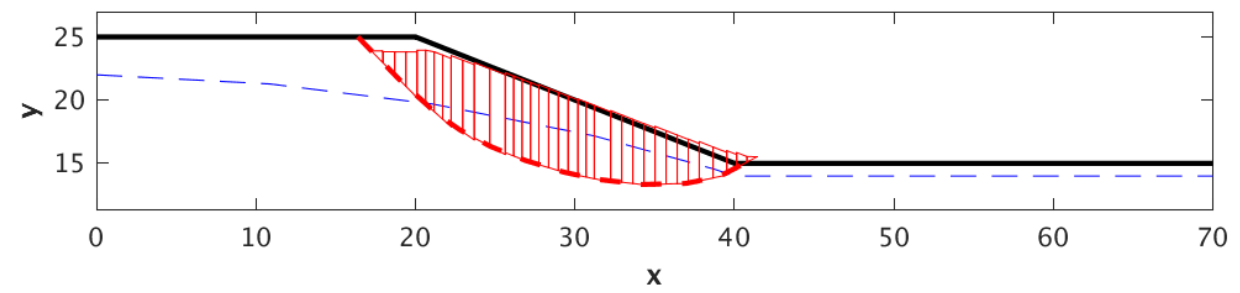
\includegraphics[width=1.0\textwidth]{OrigProgSlip.png}
		\caption{The critical slip surface for \tcref{TC_OrigProgSlip} 
		calculated by the original version of \progname{}}
		\label{OrigProgSlip}
	\end{center}
\end{figure}

How test will be performed: Automated test on unit testing framework

\item [TC\refstepcounter{testnum}\thetestnum: \label{TC_OrigProgNormal}] 
test-origProg\_normal

Control: Automatic

Initial State: New session

Input: As described in Table~\ref{ExValidInputs}, except with an additional 
slope layer described by the following coordinates: \{(0, 20), (36, 17), (40, 
15), (70, 15)\}.

Output: Relative error between the interslice normal force calculated by 
\progname{} and the interslice normal force calculated by the original version 
of \progname{}, which is assumed to be correct and can be found at 
\newline
\href{https://github.com/smiths/caseStudies/tree/master/CaseStudies/ssp/misc}
{https://github.com/smiths/caseStudies/tree/master/CaseStudies/ssp/misc}. The 
relative error will be calculated at 10 evenly spaced points spanning the 
critical slip surface and averaged to obtain the relative error to consider for 
this test case. The interslice normal forces along the critical slip surface 
calculated by the original \progname{} are shown in Figure~\ref{OrigProgForces}.

How test will be performed: Automated test on unit testing framework

\item [TC\refstepcounter{testnum}\thetestnum: \label{TC_OrigProgShear}] 
test-origProg\_shear

Control: Automatic

Initial State: New session

Input: As described in Table~\ref{ExValidInputs}, except with an additional 
slope layer described by the following coordinates: \{(0, 20), (36, 17), (40, 
15), (70, 15)\}.

Output: Relative error between the interslice shear force calculated by 
\progname{} and the interslice shear force calculated by the original version 
of \progname{}, which is assumed to be correct and can be found at 
\newline
\href{https://github.com/smiths/caseStudies/tree/master/CaseStudies/ssp/misc}
{https://github.com/smiths/caseStudies/tree/master/CaseStudies/ssp/misc}. The 
relative error will be calculated at 10 evenly spaced points spanning the 
critical slip surface and averaged to obtain the relative error to consider for 
this test case. The interslice shear forces along the critical slip surface 
calculated by the original \progname{} are shown in Figure~\ref{OrigProgForces}.

How test will be performed: Automated test on unit testing framework

\begin{figure}[h!]
	\begin{center}
		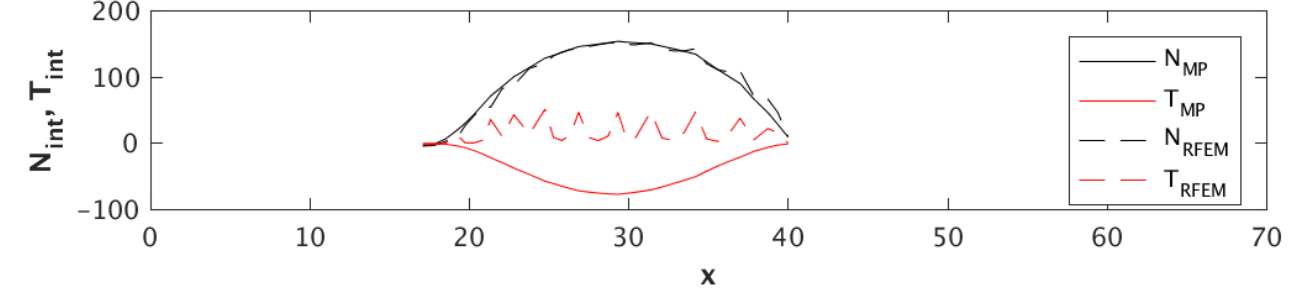
\includegraphics[width=1.0\textwidth]{OrigProgForces.png}
		\caption{The interslice normal and shear forces for 
			\tcref{TC_OrigProgNormal} and \tcref{TC_OrigProgShear} calculated 
			by the original version of \progname{}, where $N_\text{MP}$ is the 
			interslice normal force and $T_\text{MP}$ is the interslice shear 
			force}
		\label{OrigProgForces}
	\end{center}
\end{figure}

\end{enumerate}

\bmac{I wanted to add tests for the correctness NFR in Section 
\ref{sec_NFRTests} but felt that it was already covered by these functional 
requirement test cases. Is that true?}

\wss{Yes, this is true.  You can still include a heading for Correctness, but
  then point out which, already specified, tests cover this NFR.  You don't
  repeat the tests, just list their identifiers.}

\subsubsection{Output Tests}

\paragraph{Output Delivery Tests}

~\newline \noindent The following set of test cases are intended to 
verify that all expected outputs are delivered by \progname{}.

\begin{enumerate}[label=TC\arabic*:,ref={\arabic*}]
	
\item [TC\refstepcounter{testnum}\thetestnum: \label{TC_OutFS}] 
test-output\_FS

Control: Automatic

Initial State: New session

Input: As described in Table~\ref{ExValidInputs}.

Output: \progname{} reports a value for the factor of safety of the critical 
slip surface

How test will be performed: Automated test on unit testing framework

\item [TC\refstepcounter{testnum}\thetestnum: \label{TC_OutSlip}] 
test-output\_slip

Control: Automatic

Initial State: New session

Input: As described in Table~\ref{ExValidInputs}.

Output: \progname{} reports the coordinates of the critical slip surface for 
the slope.

How test will be performed: Automated test on unit testing framework

\item [TC\refstepcounter{testnum}\thetestnum: \label{TC_OutNormal}] 
test-output\_normal

Control: Automatic

Initial State: New session

Input: As described in Table~\ref{ExValidInputs}.

Output: \progname{} reports the interslice normal force along the critical slip 
surface for the slope.

How test will be performed: Automated test on unit testing framework

\item [TC\refstepcounter{testnum}\thetestnum: \label{TC_OutShear}] 
test-output\_shear

Control: Automatic

Initial State: New session

Input: As described in Table~\ref{ExValidInputs}.

Output: \progname{} reports the interslice shear force along the critical slip 
surface for the slope.

How test will be performed: Automated test on unit testing framework
	
\end{enumerate}

\paragraph{Output Verification Tests}

~\newline \noindent The following set of test cases are intended to 
verify that that the output of \progname{} obeys the physical constraints 
described in Section \ref{SRS-sec_DataConstraints} of the SRS.

\begin{enumerate}[label=TC\arabic*:,ref={\arabic*}]
	
\item [TC\refstepcounter{testnum}\thetestnum: \label{TC_ValidOutFS}] 
test-valid\_output\_FS

Control: Automatic

Initial State: New session

Input: As described in Table~\ref{ExValidInputs}.

Output: The factor of safety reported by \progname{} is greater than 0.

How test will be performed: Automated test on unit testing framework

\item [TC\refstepcounter{testnum}\thetestnum: \label{TC_ValidOutSlip}] 
test-valid\_output\_slip

Control: Automatic

Initial State: New session

Input: As described in Table~\ref{ExValidInputs}.

Output: The slope between consecutive coordinates of the critical slip surface 
are always increasing. In mathematical terms, if $j$ is an index representing a 
single coordinate and $j+1$ represents the consecutive coordinate in the 
positive $x$-direction, \newline
$\left(\frac{y_{\text{cs}_{j+2}}-y_{\text{cs}_{j+1}}}{x_{\text{cs}_{j+2}}-
		x_{\text{cs}_{j+1}}}\right)-\left(\frac{y_{\text{cs}_{j+1}}-
			y_{\text{cs}_{j}}}{x_{\text{cs}_{j+1}}-
				x_{\text{cs}_{j}}}\right) > 0$.

How test will be performed: Automated test on unit testing framework

\item [TC\refstepcounter{testnum}\thetestnum: \label{TC_ValidOutNormal}] 
test-valid\_output\_normal

Control: Automatic

Initial State: New session

Input: As described in Table~\ref{ExValidInputs}.

Output: The interslice normal forces reported by \progname{} are always greater 
than 0 across the entire critical slip surface.

How test will be performed: Automated test on unit testing framework

\item [TC\refstepcounter{testnum}\thetestnum: \label{TC_ValidOutShear}] 
test-valid\_output\_shear

Control: Automatic

Initial State: New session

Input: As described in Table~\ref{ExValidInputs}.

Output: The interslice shear forces reported by \progname{} are always less 
than 0 across the entire critical slip surface.

How test will be performed: Automated test on unit testing framework
	
\end{enumerate}

\subsection{Tests for Nonfunctional Requirements} \label{sec_NFRTests}

\subsubsection{Maintainability Test} \label{sec_Maintainability}

\begin{enumerate}[label=TC\arabic*:,ref={\arabic*}]
	
\item [TC\refstepcounter{testnum}\thetestnum: \label{TC_Maintainability}] 
test-maintainability

Type: Manual
					
Initial State: Test subject has a completed MG for \progname{}
					
Input/Condition: MG for \progname{} and the following question "If you were 
tasked with modifying \progname{} to accept an imposed surface load as an input 
and incorporate this additional force into the computation, which module(s) 
would you change?"
					
Output/Result: Input Module, Input Verification Module, Calculation Module

\bmac{Subject to change since design has not been completed yet}
					
How test will be performed: Test subject will be asked the question described 
in "Input/Condition" and must answer only by consulting the MG. Their answer 
will be recorded and compared with the correct answer outlined in 
"Output/Result". If the subject answers correctly, the test passes and 
confidence in the maintainability of \progname{} is increased. If the subject 
answers incorrectly, the test fails and the documentation or implementation of 
\progname{} must be updated to be more maintainable.
					
\end{enumerate}

\wss{I like these tests!}

\subsubsection{Reusability Test} \label{sec_Reusability}

\begin{enumerate}[label=TC\arabic*:,ref={\arabic*}]
	
\item [TC\refstepcounter{testnum}\thetestnum: \label{TC_Reusability}] 
test-reusability

Type: Manual

Initial State: There is a completed implementation of \progname{}
	
Input/Condition: Code that prompts the user for command-line inputs related to 
slope stability analysis.

Output/Result: An alternative version of \progname{} that uses the input code. 
All modules in the alternative version should be identical to the existing 
\progname{} modules, with the exception of the Input Module.

How test will be performed: The alternative version of \progname{} will be 
developed by Brooks MacLachlan. If only the Input Module is changed from the 
existing version, then the test passes and confidence in the reusability of 
\progname{}'s modules is increased. If other modules need to be changed, the 
test fails and the other modules must be modified to be completely reusable.
	
\end{enumerate}

\subsubsection{Correctness Tests}
The correctness NFR is covered by the functional requirement test cases for 
calculations, found in 
Section~\ref{sec_CalcTCs}.

\subsubsection{Understandability Tests}
Understandability is a contributing factor to maintainability and reusability. 
Therefore, the understandability NFR is covered by the test cases for 
maintainability and reusability, found in Section~\ref{sec_Maintainability} and 
Section~\ref{sec_Reusability}, respectively.

\subsection{Traceability Between Test Cases and Requirements}

\noindent The purpose of the traceability matrix shown in 
Table~\ref{Table:T_trace} and Table~\ref{Table:NFR_trace} is to provide easy 
references on which requirements are verified by which test cases, and which 
test cases need to be updated if a requirement changes.  If a requirement is 
changed, the items in the column of that requirement that are marked
with an ``X'' may have to be modified as well. 

\begin{table}[!h]
	\centering
	\begin{tabular}{|c|c|c|c|c|c|c|c|c|c|c|}
		\hline
		& \rref{SRS-R_Inputs}& \rref{SRS-R_KinAdm}& \rref{SRS-R_InitGen}& 
		\rref{SRS-R_FS}& \rref{SRS-R_Minimize} & \rref{SRS-R_VerifyOutput}& 
		\rref{SRS-R_CritGraph}& \rref{SRS-R_OutputFS}& 
		\rref{SRS-R_NormalGraph}& \rref{SRS-R_ShearGraph} \\
		\hline
		\tcref{TC_ValidInDec} - \tcref{TC_ValidInXMaxEndEqual}                 
		& X& & & & & & & & & \\ \hline
		\tcref{TC_InvalidSlopeDecToInc} - \tcref{TC_InvalidUnitWtWaterNegative} 
		& & X& & & & & & & & \\ \hline
		\tcref{TC_Ex1FS} - \tcref{TC_OrigProgSlip}                             
		& & & X& X& X& & & & & \\ \hline
		\tcref{TC_OrigProgNormal}                                              
		& & & & & & & & & X& \\ \hline
		\tcref{TC_OrigProgShear}                                               
		& & & & & & & & & & X\\ \hline
		\tcref{TC_OutFS}                                                       
		& & & & & & & X& & & \\ \hline
		\tcref{TC_OutSlip}                                                     
		& & & & & & & & X& & \\ \hline
		\tcref{TC_OutNormal}                                                   
		& & & & & & & & & X& \\ \hline
		\tcref{TC_OutShear}                                                    
		& & & & & & & & & & X \\ \hline
		\tcref{TC_ValidOutFS} - \tcref{TC_ValidOutShear}                        
		& & & & & & X& & & & \\
		\hline
	\end{tabular}
	\caption{Traceability Matrix Showing the Connections Between Functional 
	Requirements and Test Cases}
	\label{Table:T_trace}
\end{table}

\begin{table}[!h]
	\centering
	\begin{tabular}{|c|c|c|c|c|}
		\hline
		& \nfrref{SRS-NFR_Correctness}& \nfrref{SRS-NFR_Understandability}& 
		\nfrref{SRS-NFR_Reusability}& \nfrref{SRS-NFR_Maintainability} \\
		\hline
		\tcref{TC_Ex1FS} - \tcref{TC_OrigProgShear}                             
		& X& & & \\ \hline
		\tcref{TC_Maintainability}                                            
		& & X& &X \\ \hline
		\tcref{TC_Reusability}                     
		& & X& X& \\
		\hline
	\end{tabular}
	\caption{Traceability Matrix Showing the Connections Between Non-Functional 
	Requirements and Test Cases}
	\label{Table:NFR_trace}
\end{table}

\wss{I had to recompile the SRS to get the table references to work.  Could you add a makefile
  to the SSP example, like the Blank Project example, so that compiling the
  example would work via make?}

\section{Static Verification Techniques} \label{sec_Static}

The reviews described in Section \ref{sec_ImpPlan} will employ the static 
verification techniques of code walkthroughs and code inspection to attempt to 
uncover issues with the implementation.

\wss{I should modify the template to remove this section, since you are correct
  that you already discussed these topics.  You can remove this section in your
  version.  You don't actually propose code walkthroughs in Section 4.4, so the
  text here isn't quite correct.}
				
\newpage

\bibliographystyle {plainnat}
\bibliography {../../../refs/References}

%\newpage

%\section{Appendix}
%
%This is where you can place additional information.
%
%\subsection{Symbolic Parameters}
%
%The definition of the test cases will call for SYMBOLIC\_CONSTANTS.
%Their values are defined in this section for easy maintenance.
%
%\subsection{Usability Survey Questions?}
%
%\wss{This is a section that would be appropriate for some projects.}

\end{document}